\documentclass[10pt,english]{article}
\usepackage{bookmark}
\usepackage{geometry}
\usepackage{anyfontsize}
\usepackage{lmodern}
\usepackage{lipsum}
\usepackage{sectsty}
\usepackage{amsmath}
\usepackage{amssymb}
\usepackage[T1]{fontenc}
\usepackage[utf8]{inputenc}
\usepackage[explicit]{titlesec}
\usepackage[sfdefault]{inter}
\usepackage{sfmath}
\usepackage{hyperref}
\usepackage{enumitem}
\usepackage{listings}
\usepackage[final]{graphicx}
\usepackage{subfig}
\usepackage{array}
\usepackage[table]{xcolor}
\usepackage{csvsimple}
\graphicspath{{./images/}}
\usepackage[explicit]{titlesec}


\linespread{1.2}
\title{\huge{\textbf{Spotting}}}
\author{
    \\\\
    David Hermanto\\
    \small 3808127\\
    \\
    Rafat Mahiuddin\\
    \small 3897093\\
    \\
    Harry Porter\\
    \small 3888604\\
    \\
    Adrian Rebellato\\
    \small 3889401\\
    \\
    Myeonghoon Sun\\
    \small 3774430\\
    \\\\
}
\date{}

\begin{document}

\maketitle
\thispagestyle{empty}
\clearpage

\vspace*{\fill}
\begin{center}
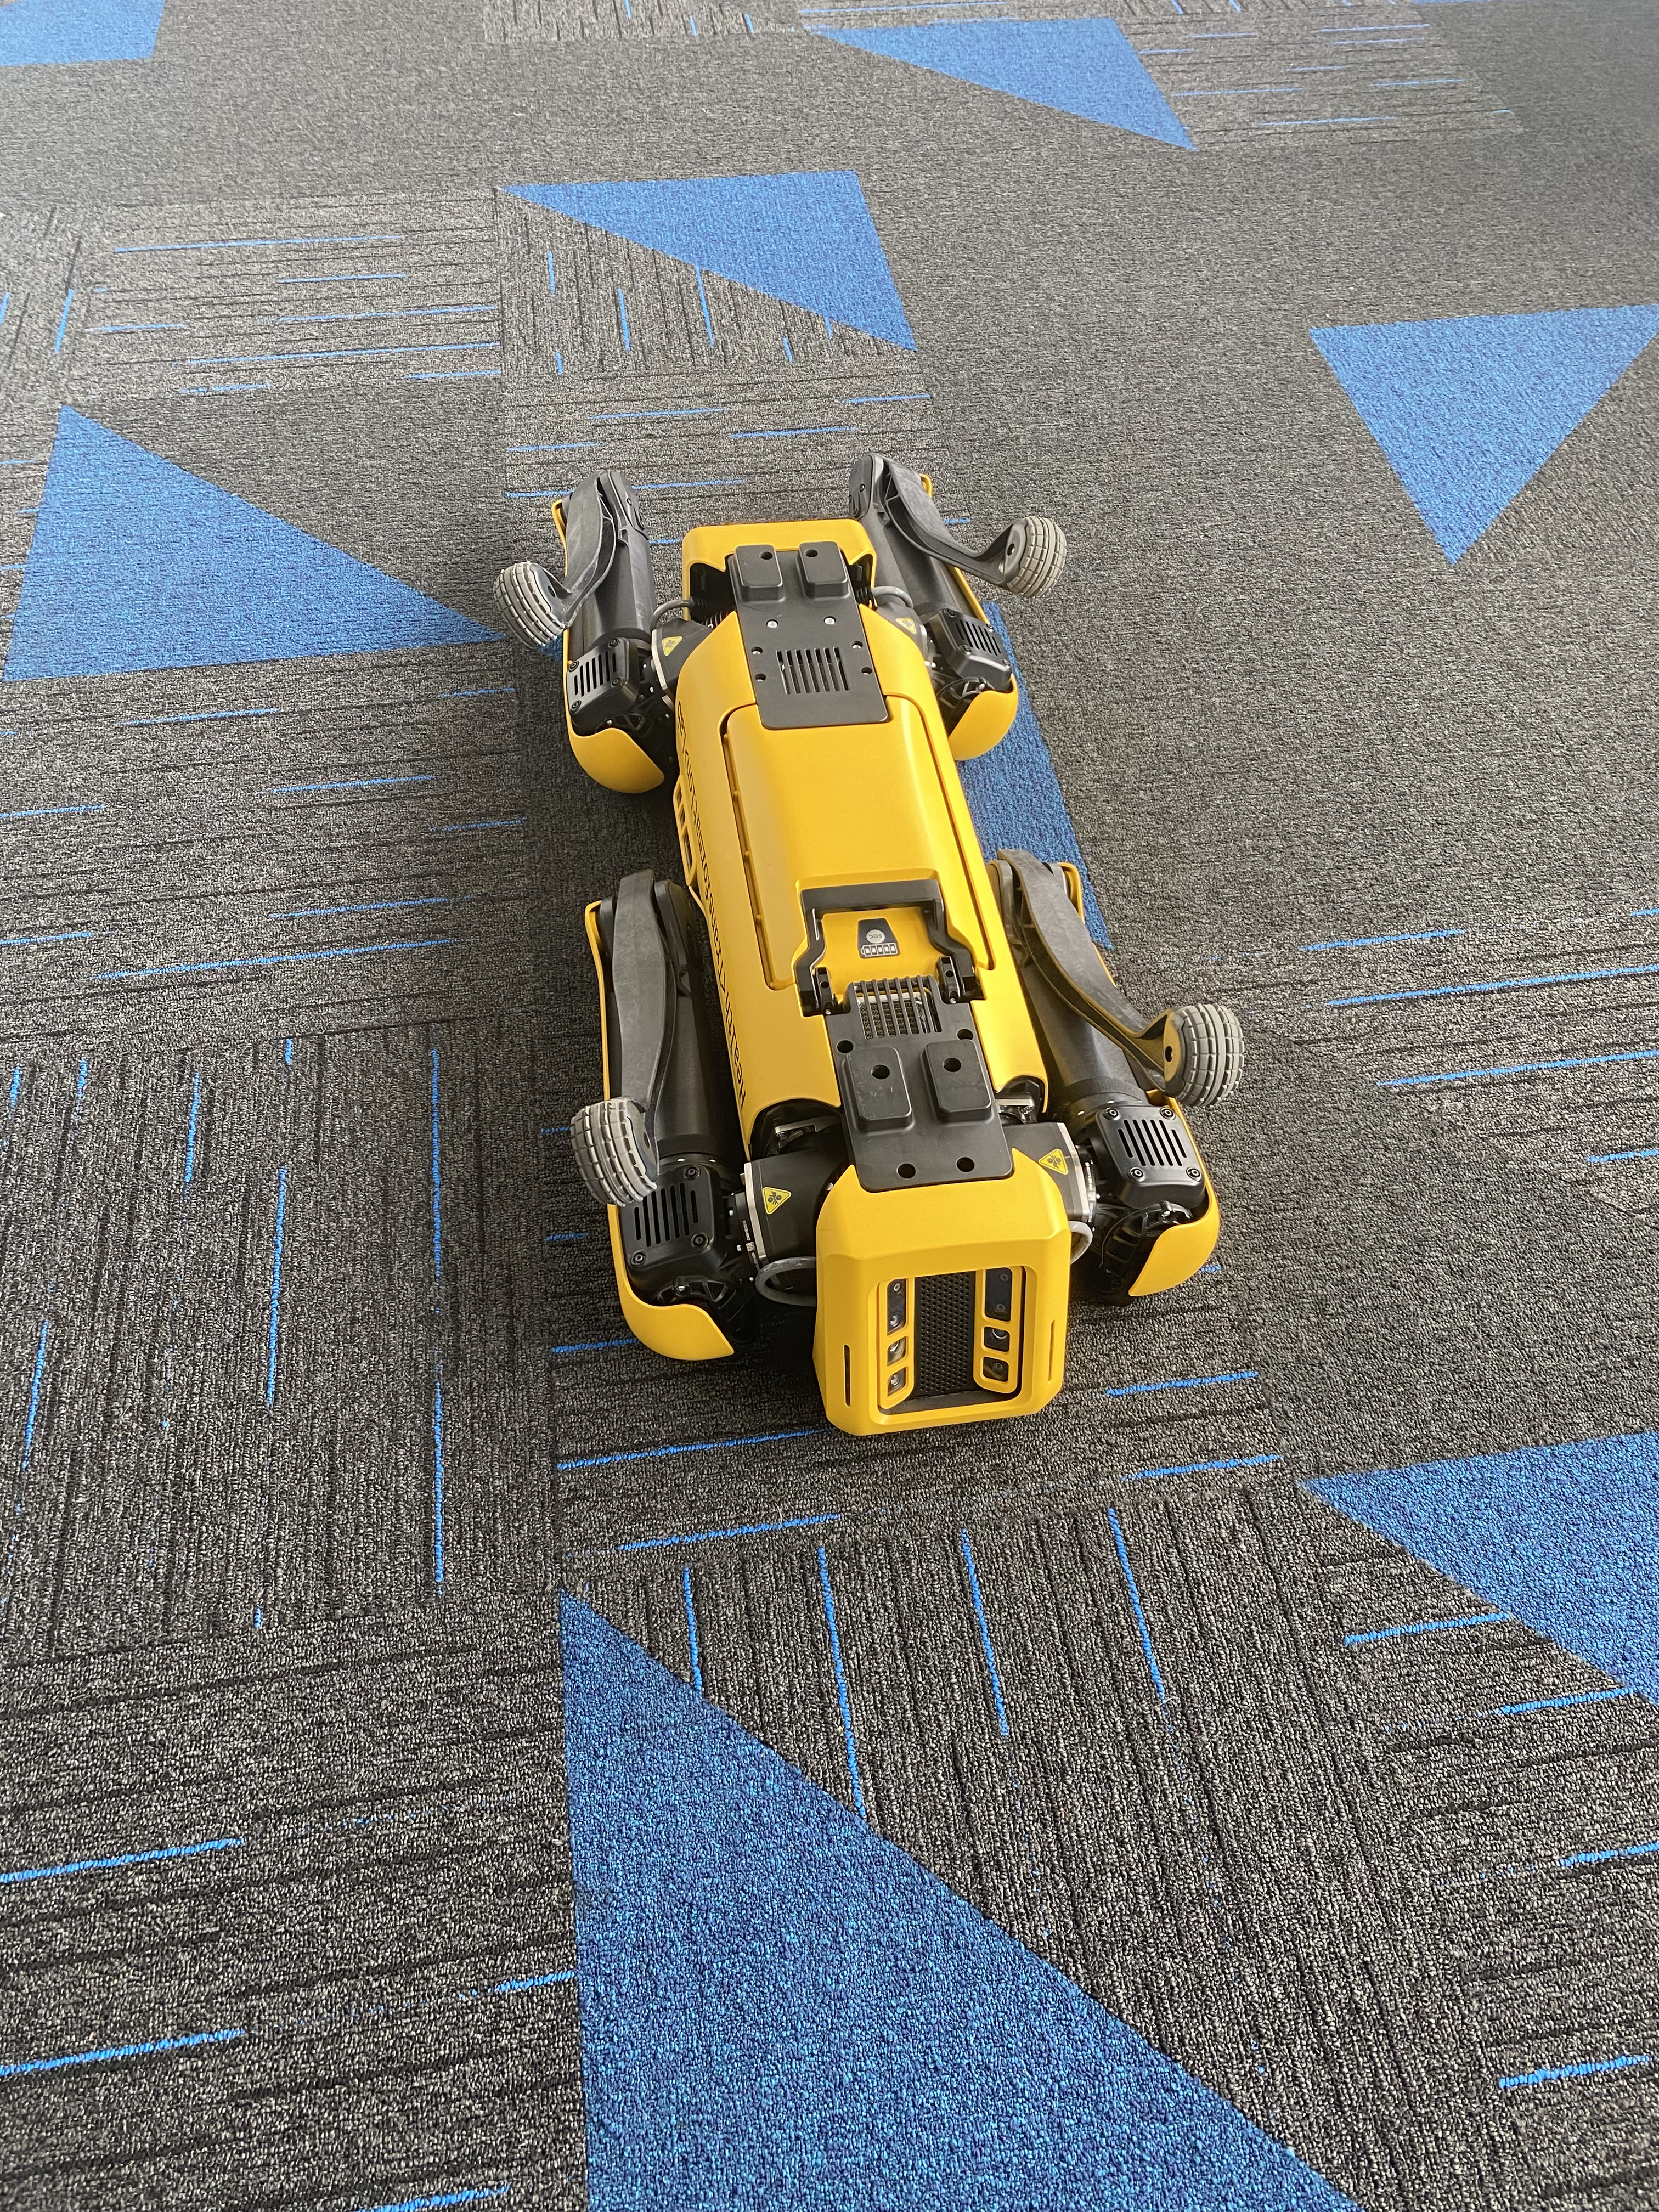
\includegraphics[scale=0.1]{images/9DDC331C-9A71-4E19-AECC-54D8ED6C2240.png}
\end{center}
\vfill
\thispagestyle{empty}

\clearpage

\pagenumbering{arabic}

\section*{Solution}

Here, we first discuss the structure and architecture of our software, then our methodology with respect to meeting the project requirements.

% Where should this go? Probably interspersed throughout the report.
% Positions the work within the literature.
% Compares the project to other appropriate state-of-the art methods.

\subsection*{Structure}

% Technical description of project:
% Software, launch files, configuration, and implementation.
% Description of the implemented software.
%   Requires:
%   - Excellent and complete technical description of the ROS package components.

\clearpage

\subsection*{Architecture}

% Description of the of Robot Software Architecture.
% Excellent and complete.

% Justification of the choice of Robot Software Architecture.
%   Requires:
%   - Excellent justification of the Robot Software Architecture.
%   - Well-supported reasoning.

\clearpage

\subsection*{Methodology}

% Describe methodology and approach towards completing the negotiated requirements of the project.
%   Requires:
%   - Excellent description of methodology.
%   - Provides a complete picture of how the project is completed.

\clearpage

\section*{Retrospective}
\clearpage

\subsection*{Analysis}

% Analysis of the strengths and weaknesses of the software.
%   Requires:
%   - Excellent analysis of the final deliverable.
%   - Provides a clear understanding of the strengths and weakness of the software.

\clearpage

\subsection*{Evaluation}

% Critical evaluation of the project in relation to the negotiated requirements.
% Quality of quantitative and/or qualitative experimental results.
%   Requires:
%   - Excellent evaluation of the capabilities of the final deliverable.
%   - Well-supported experimental evidence.

\clearpage

\subsection*{Improvements}
\clearpage

\vspace*{\fill}
\begin{center}
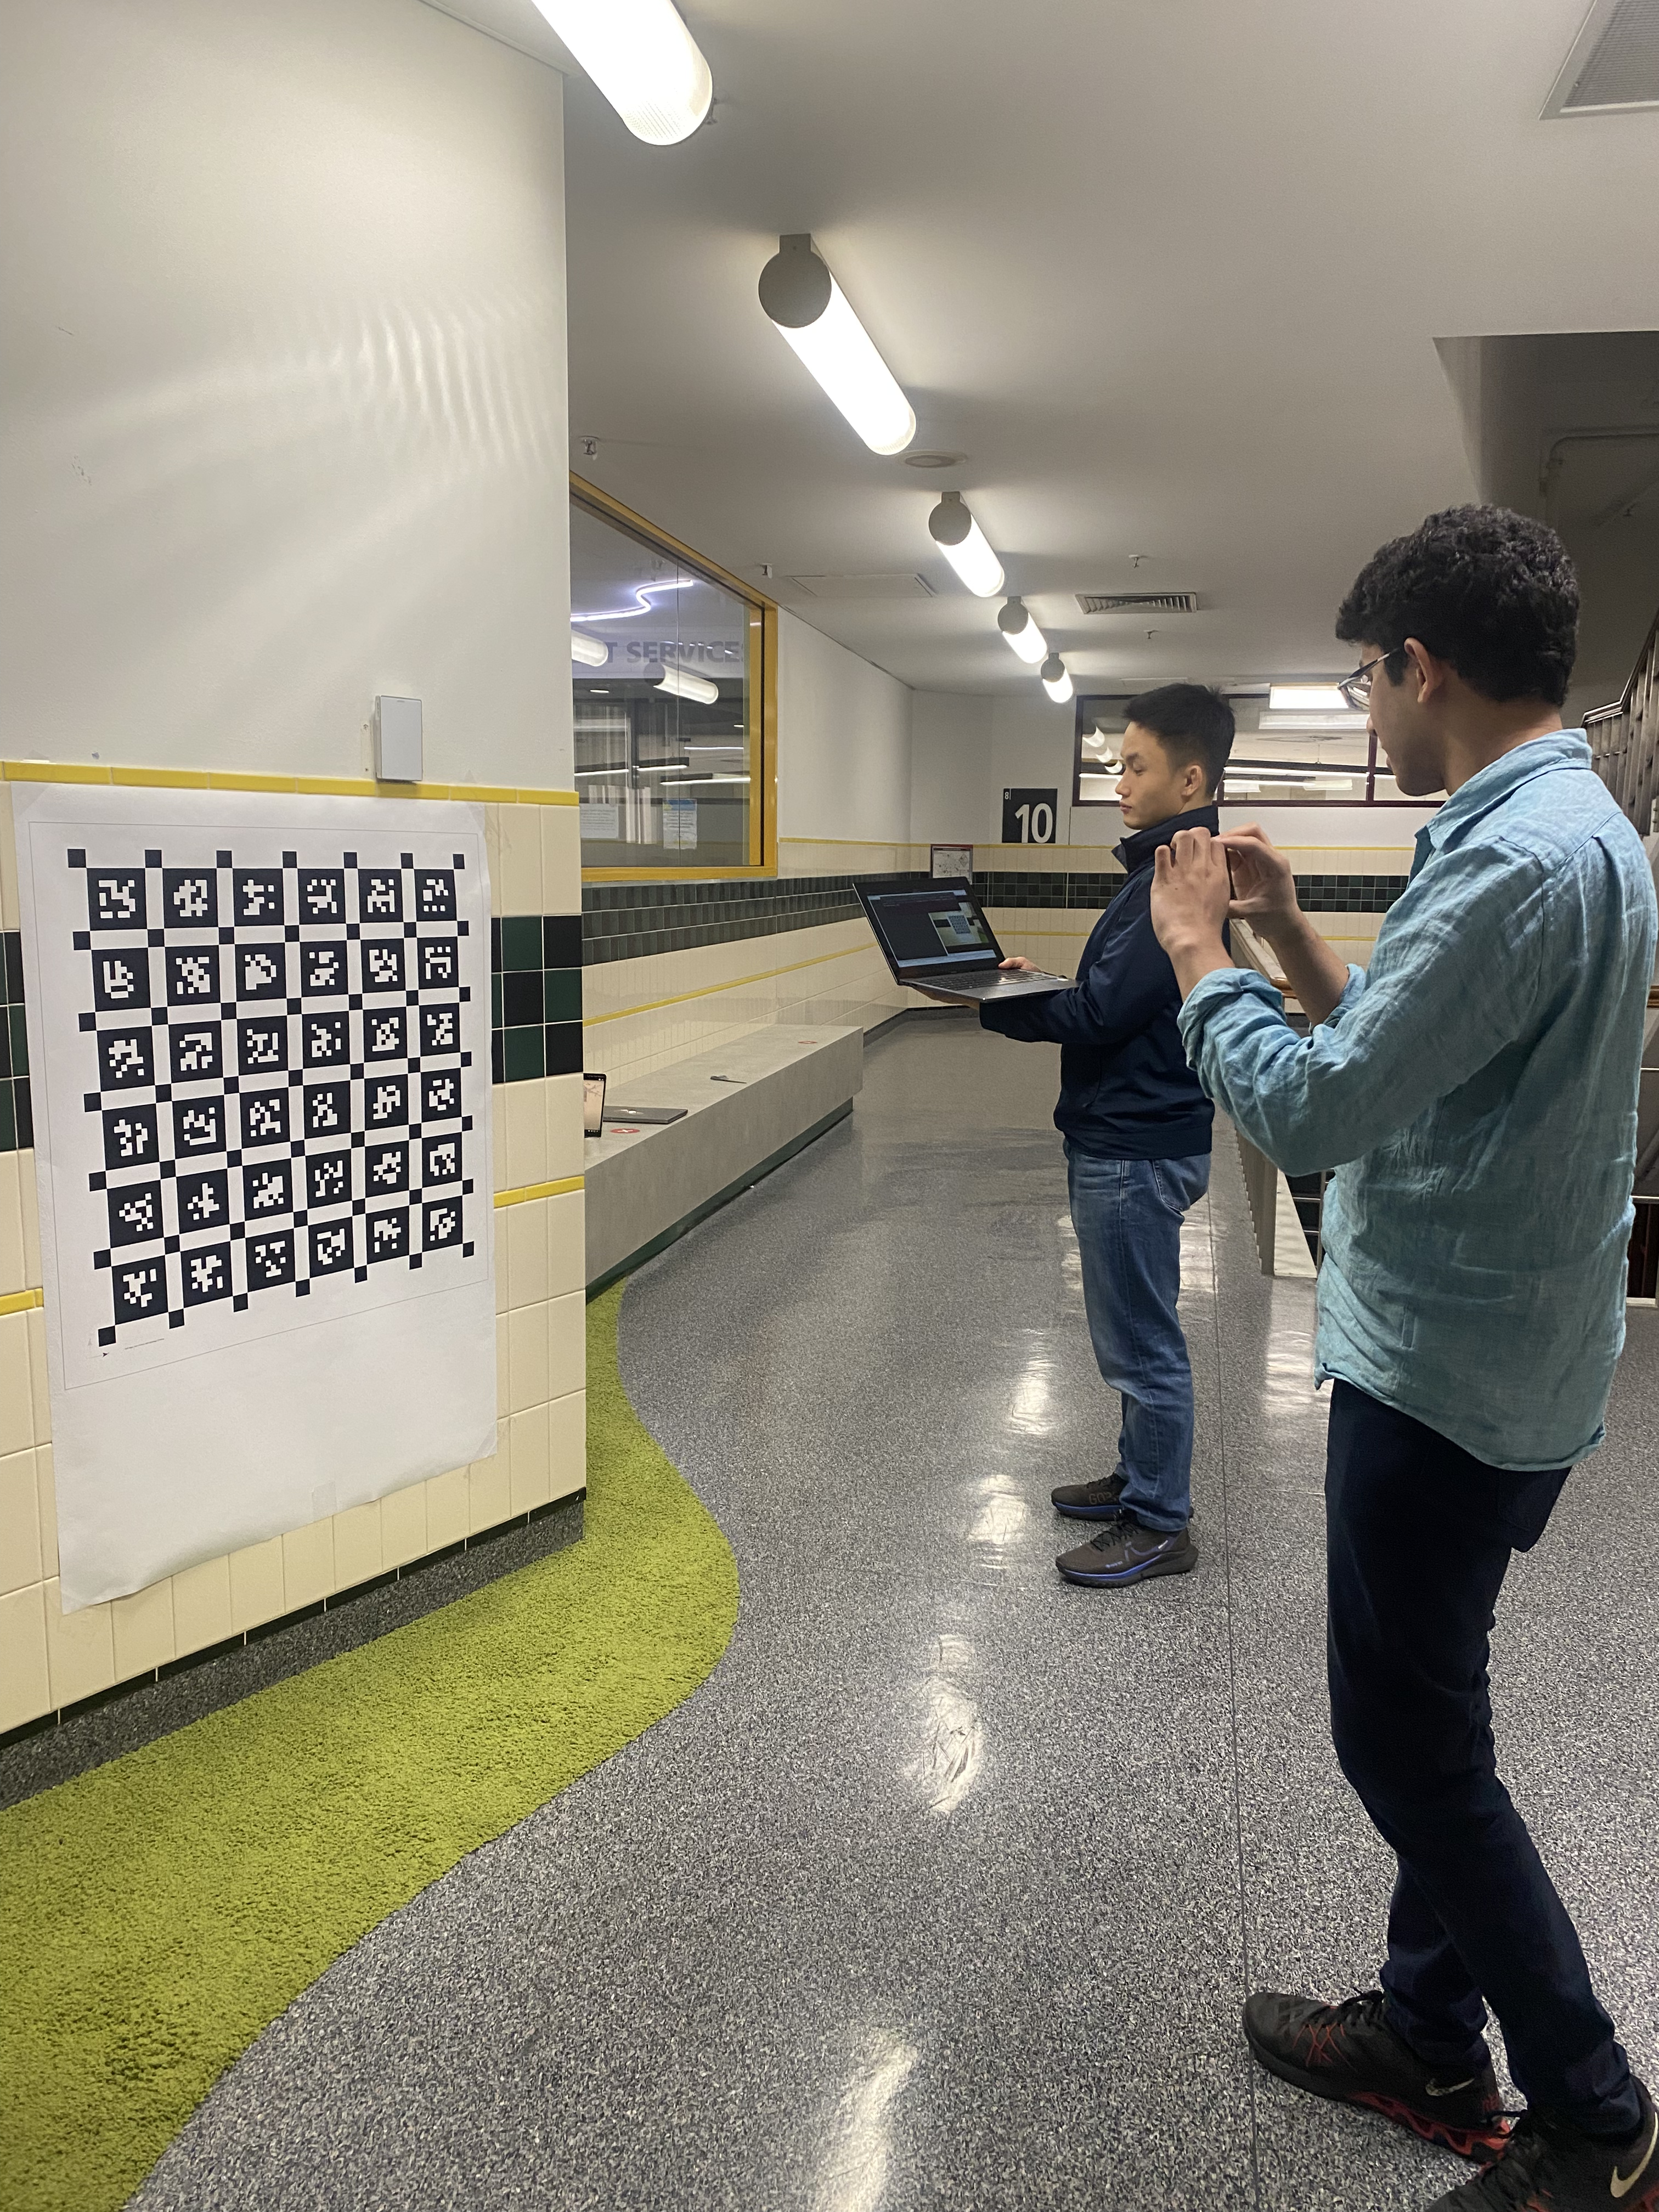
\includegraphics[scale=0.1]{images/429F1310-292D-47FB-AB48-3564D69C3279.png}
\end{center}
\vfill
\thispagestyle{empty}
\clearpage

\section*{Contributions}
\clearpage

\section*{References}

\begin{enumerate}[leftmargin=*,label={\texttt{[\arabic*]}},noitemsep]
    \item P. E. Teleweck and B. Chandrasekaran, “Path planning algorithms and their use in robotic navigation systems,” Journal of Physics: Conference Series, vol. 1207, p. 012018, 2019. doi:10.1088/1742-6596/1207/1/012018
\end{enumerate}

\end{document}
